\section{DIL\_\-Visualize\_\-with\_\-HTML\_\-Tabs  Class Reference}
\label{classDIL__Visualize__with__HTML__Tabs}\index{DIL_Visualize_with_HTML_Tabs@{DIL\_\-Visualize\_\-with\_\-HTML\_\-Tabs}}
{\tt \#include $<$dil2al.hh$>$}

Inheritance diagram for DIL\_\-Visualize\_\-with\_\-HTML\_\-Tabs::\begin{figure}[H]
\begin{center}
\leavevmode
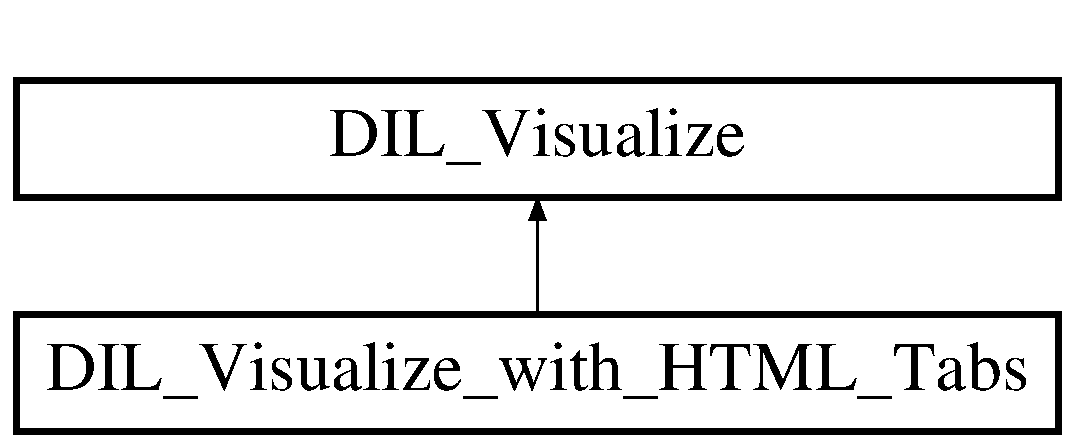
\includegraphics[height=2cm]{classDIL__Visualize__with__HTML__Tabs}
\end{center}
\end{figure}
\subsection*{Public Methods}
\begin{CompactItemize}
\item 
{\bf DIL\_\-Visualize\_\-with\_\-HTML\_\-Tabs} ({\bf DIL\_\-Hierarchy\_\-Level\_\-Data} $\ast$ld=NULL)
\item 
virtual void {\bf Initialize} ()
\item 
virtual void {\bf Visualize\_\-Element} ({\bf DIL\_\-entry} $\ast$de, int depth)
\item 
virtual void {\bf Visualize\_\-Not\-Shown} (int numdependencies, int depth)
\item 
virtual {\bf String} {\bf Output} ()
\item 
virtual {\bf String} {\bf Output\_\-Content} ()
\end{CompactItemize}
\subsection*{Protected Attributes}
\begin{CompactItemize}
\item 
{\bf String} {\bf s}
\item 
{\bf String} {\bf content}
\end{CompactItemize}


\subsection{Constructor \& Destructor Documentation}
\index{DIL_Visualize_with_HTML_Tabs@{DIL\_\-Visualize\_\-with\_\-HTML\_\-Tabs}!DIL_Visualize_with_HTML_Tabs@{DIL\_\-Visualize\_\-with\_\-HTML\_\-Tabs}}
\index{DIL_Visualize_with_HTML_Tabs@{DIL\_\-Visualize\_\-with\_\-HTML\_\-Tabs}!DIL_Visualize_with_HTML_Tabs@{DIL\_\-Visualize\_\-with\_\-HTML\_\-Tabs}}
\subsubsection{\setlength{\rightskip}{0pt plus 5cm}DIL\_\-Visualize\_\-with\_\-HTML\_\-Tabs::DIL\_\-Visualize\_\-with\_\-HTML\_\-Tabs ({\bf DIL\_\-Hierarchy\_\-Level\_\-Data} $\ast$ {\em ld} = NULL)\hspace{0.3cm}{\tt  [inline]}}\label{classDIL__Visualize__with__HTML__Tabs_a0}




Definition at line 780 of file dil2al.hh.



\footnotesize\begin{verbatim}780 : DIL_Visualize(ld) {}
\end{verbatim}\normalsize 


\subsection{Member Function Documentation}
\index{DIL_Visualize_with_HTML_Tabs@{DIL\_\-Visualize\_\-with\_\-HTML\_\-Tabs}!Initialize@{Initialize}}
\index{Initialize@{Initialize}!DIL_Visualize_with_HTML_Tabs@{DIL\_\-Visualize\_\-with\_\-HTML\_\-Tabs}}
\subsubsection{\setlength{\rightskip}{0pt plus 5cm}virtual void DIL\_\-Visualize\_\-with\_\-HTML\_\-Tabs::Initialize ()\hspace{0.3cm}{\tt  [inline, virtual]}}\label{classDIL__Visualize__with__HTML__Tabs_a1}




Reimplemented from {\bf DIL\_\-Visualize} {\rm (p.\,\pageref{classDIL__Visualize_a1})}.

Definition at line 781 of file dil2al.hh.



\footnotesize\begin{verbatim}781 { s = ""; content = ""; }
\end{verbatim}\normalsize 
\index{DIL_Visualize_with_HTML_Tabs@{DIL\_\-Visualize\_\-with\_\-HTML\_\-Tabs}!Output@{Output}}
\index{Output@{Output}!DIL_Visualize_with_HTML_Tabs@{DIL\_\-Visualize\_\-with\_\-HTML\_\-Tabs}}
\subsubsection{\setlength{\rightskip}{0pt plus 5cm}virtual {\bf String} DIL\_\-Visualize\_\-with\_\-HTML\_\-Tabs::Output ()\hspace{0.3cm}{\tt  [inline, virtual]}}\label{classDIL__Visualize__with__HTML__Tabs_a4}




Reimplemented from {\bf DIL\_\-Visualize} {\rm (p.\,\pageref{classDIL__Visualize_a7})}.

Definition at line 784 of file dil2al.hh.

Referenced by Tabbed\_\-HTML\_\-DIL\_\-Hierarchy().



\footnotesize\begin{verbatim}784 { return s; }
\end{verbatim}\normalsize 
\index{DIL_Visualize_with_HTML_Tabs@{DIL\_\-Visualize\_\-with\_\-HTML\_\-Tabs}!Output_Content@{Output\_\-Content}}
\index{Output_Content@{Output\_\-Content}!DIL_Visualize_with_HTML_Tabs@{DIL\_\-Visualize\_\-with\_\-HTML\_\-Tabs}}
\subsubsection{\setlength{\rightskip}{0pt plus 5cm}virtual {\bf String} DIL\_\-Visualize\_\-with\_\-HTML\_\-Tabs::Output\_\-Content ()\hspace{0.3cm}{\tt  [inline, virtual]}}\label{classDIL__Visualize__with__HTML__Tabs_a5}




Definition at line 785 of file dil2al.hh.

Referenced by Tabbed\_\-HTML\_\-DIL\_\-Hierarchy().



\footnotesize\begin{verbatim}785 { return content; }
\end{verbatim}\normalsize 
\index{DIL_Visualize_with_HTML_Tabs@{DIL\_\-Visualize\_\-with\_\-HTML\_\-Tabs}!Visualize_Element@{Visualize\_\-Element}}
\index{Visualize_Element@{Visualize\_\-Element}!DIL_Visualize_with_HTML_Tabs@{DIL\_\-Visualize\_\-with\_\-HTML\_\-Tabs}}
\subsubsection{\setlength{\rightskip}{0pt plus 5cm}void DIL\_\-Visualize\_\-with\_\-HTML\_\-Tabs::Visualize\_\-Element ({\bf DIL\_\-entry} $\ast$ {\em de}, int {\em depth})\hspace{0.3cm}{\tt  [virtual]}}\label{classDIL__Visualize__with__HTML__Tabs_a2}




Reimplemented from {\bf DIL\_\-Visualize} {\rm (p.\,\pageref{classDIL__Visualize_a5})}.

Definition at line 121 of file diladmin.cc.

References DIL\_\-ID::chars(), content, DIL\_\-Topical\_\-List::dil, Elipsis\_\-At(), DIL\_\-entry::Entry\_\-Text(), filetitle\_\-t::file, String::gsub(), HTML\_\-put\_\-href(), HTML\_\-remove\_\-tags(), replicate(), s, and DIL\_\-entry::Topics().



\footnotesize\begin{verbatim}121                                                                               {
122   String ptxtcontent;
123   content += "\nDIL#" + String(de->chars()) + ":\n";
124   String * ctxt = de->Entry_Text();
125   if (ctxt) {
126     ptxtcontent = (*ctxt);
127     content += (*HTML_remove_tags(ptxtcontent));
128     Elipsis_At(ptxtcontent,hierarchyexcerptlength);
129     ptxtcontent.gsub('\n',' ');
130   } else ptxtcontent = "<!-- excerpt requires content file option -->";
131   content += '\n';
132   if (depth>0) s += replicate('\t',depth);
133   s += HTML_put_href((de->Topics(0)->dil.file+'#')+de->chars(),"DIL#" + String(de->chars())) + ": " + ptxtcontent + '\n';
134 }
\end{verbatim}\normalsize 
\index{DIL_Visualize_with_HTML_Tabs@{DIL\_\-Visualize\_\-with\_\-HTML\_\-Tabs}!Visualize_NotShown@{Visualize\_\-NotShown}}
\index{Visualize_NotShown@{Visualize\_\-NotShown}!DIL_Visualize_with_HTML_Tabs@{DIL\_\-Visualize\_\-with\_\-HTML\_\-Tabs}}
\subsubsection{\setlength{\rightskip}{0pt plus 5cm}void DIL\_\-Visualize\_\-with\_\-HTML\_\-Tabs::Visualize\_\-Not\-Shown (int {\em numdependencies}, int {\em depth})\hspace{0.3cm}{\tt  [virtual]}}\label{classDIL__Visualize__with__HTML__Tabs_a3}




Reimplemented from {\bf DIL\_\-Visualize} {\rm (p.\,\pageref{classDIL__Visualize_a6})}.

Definition at line 136 of file diladmin.cc.

References replicate(), and s.



\footnotesize\begin{verbatim}136                                                                                     {
137   if (numdependencies>0) {
138     if (depth>0) s += replicate('\t',depth);
139     s += '['+String((long) numdependencies);
140     if (reversehierarchy) s += " superiors...]\n";
141     else s += " dependencies...]\n";
142   }
143 }
\end{verbatim}\normalsize 


\subsection{Member Data Documentation}
\index{DIL_Visualize_with_HTML_Tabs@{DIL\_\-Visualize\_\-with\_\-HTML\_\-Tabs}!content@{content}}
\index{content@{content}!DIL_Visualize_with_HTML_Tabs@{DIL\_\-Visualize\_\-with\_\-HTML\_\-Tabs}}
\subsubsection{\setlength{\rightskip}{0pt plus 5cm}{\bf String} DIL\_\-Visualize\_\-with\_\-HTML\_\-Tabs::content\hspace{0.3cm}{\tt  [protected]}}\label{classDIL__Visualize__with__HTML__Tabs_n1}




Definition at line 778 of file dil2al.hh.

Referenced by Visualize\_\-Element().\index{DIL_Visualize_with_HTML_Tabs@{DIL\_\-Visualize\_\-with\_\-HTML\_\-Tabs}!s@{s}}
\index{s@{s}!DIL_Visualize_with_HTML_Tabs@{DIL\_\-Visualize\_\-with\_\-HTML\_\-Tabs}}
\subsubsection{\setlength{\rightskip}{0pt plus 5cm}{\bf String} DIL\_\-Visualize\_\-with\_\-HTML\_\-Tabs::s\hspace{0.3cm}{\tt  [protected]}}\label{classDIL__Visualize__with__HTML__Tabs_n0}




Definition at line 777 of file dil2al.hh.

Referenced by Visualize\_\-Element(), and Visualize\_\-Not\-Shown().

The documentation for this class was generated from the following files:\begin{CompactItemize}
\item 
{\bf dil2al.hh}\item 
{\bf diladmin.cc}\end{CompactItemize}
